\documentclass[11pt,a4paper]{article}

% [†ONT-SIM] EMPIRICAL-FOLIATION / SIMULTANEITY FORCING — this paper is the HOME (ONTOLOGY_FOUNDATION_INDEX.md §1d).
%   Masthead / established here (the empirical hinge of the programme): the cosmological redshift is the
%   path integral of the expansion rate, so the CMB monopole isotropy is a DIRECT MEASUREMENT of uniform
%   expansion (isotropy-from-homogeneity is a category error); a matter-tracking expansion would scatter
%   redshift ~1e-2 (8.9e-3 for uncorrelated cells, the most accommodating case), more than 200x the whole
%   measured CMB anisotropy 4.1e-5 => the cosmic foliation is MEASURED, not assumed ("the modern
%   parallax"). Read ontologically (thm:augmentation): the foliation is the lapse
%   (the objective present), synchrony's relativity the shift; reading synchrony-relativity as
%   no-objective-present is a MODAL FALLACY the isotropy falsifies. Synchrony relative; simultaneity
%   ABSOLUTE and measured. This is the empirical rung of P7's cosmic-time commitment and p0's maximal
%   symmetry, the measured counterpart of the Tier-C essays. Do not concede the relational "no preferred
%   frame / no objective now" default — P4 falsified it.
%
% [†ONT-EPI] The modal fallacy this paper falsifies is established as a theorem (thm:modal) in the
%   companion epistemic paper (P6), held whole in ONTOLOGY_FOUNDATION_INDEX.md §1g — which also
%   licenses the method's warrant (R2 / least-arbitrariness) this paper leans on, and marks the
%   altitude a forcing is claimed at. P6 supplies the LOGIC; this paper supplies the
%   non-local MEASUREMENT that decides it. Per P6 §place, this paper is where the programme first
%   leans on the method.
%
% =====================================================================
% SPINE POSITION — P4.
%   This paper is P4 (modern_parallax), the empirical/physics-first
%   foundation, ahead of P5 groupoid_paper (which supplies the algebraic
%   content of the augmentation established here), P6 shadow_of_existence
%   and P7 CR_framework: the empirical forcing precedes its algebra.
%   Citations are key-based; authoritative numbering: CORPUS_MAP.md.
%
% It is the empirical-and-ontological FOUNDATION that opens the dynamic
% half: the redshift-isotropy floor forcing cosmic time and uniform
% expansion. This paper carries the
% logical/categorical/ontological closure of CR's adjudicated distinctions
% — occurrence/existence (the lapse) and the relativity of synchrony vs the
% absoluteness of simultaneity (the shift) — as a structural THEOREM in
% sec:augmentation (thm:augmentation): CR is the NECESSARY AND SUFFICIENT
% augmentation of GR for a coherent formal description of an existing,
% evolving world — the completion of the two-part Newton--Einstein formalism
% the standard reading left fused. Dug from the ontology resources
% (conceptual-boundary essays + canonical_time). The theorem is dropped here,
% before P8 formalizes; the forced geometric details (dS substrate, the cut,
% the bend) are the back half's, the minimal-structure uniqueness the book's.
% Green-Wald is read in sec:tension as STABILITY, not existence: it
% presupposes the foliation the floor forces, so the backreaction dispute
% (Buchert et al vs Green-Wald) is settled structurally from outside (sec:establishes).
% ORDER: the question (density sets the rate?) -> how the principle entered
% (sec:history, sec:order, sec:twoforms) -> the challenge (sec:challenge) ->
% the observable (sec:decomp) -> the test (sec:floor) -> sec:establishes ->
% sec:stands -> what follows (sec:follows).
% CANON NOTE — ontology live. CR is ontological: the real 3-space (the layer)
% EXISTS and advances in cosmic time; the 4-manifold records what happens.
% "Uniform expansion" is the layer's advance, not a property of a block.
% The cosmic foliation established here is a MEASURED feature of the world,
% not a coordinate convenience.
%
% REFERENCES: the load-bearing standard-model claims are sourced from primary
% literature -- Hubble 1929; Robertson 1933/1935; Walker 1937; North 1965;
% Eddington 1920; Friedmann 1922; Lemaitre 1927; Sachs--Wolfe 1967; Ellis 1971;
% Barrett--Clarkson 2000; Clarkson--Bassett--Lu 2008; Maartens 2011; Rasanen 2009;
% Planck 2018 (parameters and power spectra); CAMB (Lewis et al. 2000) -- plus
% the expansion-history tracers Eisenstein 2005 (BAO standard ruler) and
% Riess 1998 + Perlmutter 1999 (SNe Ia standard candles).
% =====================================================================

\usepackage[margin=1in]{geometry}
\usepackage{amsmath, amssymb, amsthm}
\usepackage{mathtools}
\usepackage{mathrsfs}
\usepackage{graphicx}
\usepackage[dvipsnames]{xcolor}
\usepackage{hyperref}
\usepackage{receipts}
\usepackage{ledgers}  % in-place receipt citations -> Appendix R
\usepackage{caption}
\newtheorem{theorem}{Theorem}

\title{The modern parallax:\\
\large the redshift-isotropy floor, the empirical forcing of cosmic time and uniform expansion,\\
and the measured resolution of the relativity of simultaneity}
\author{Daryl Janzen\\
\small Department of Physics and Engineering Physics\\
\small University of Saskatchewan}
\date{}

\begin{document}
\maketitle

\begin{abstract}
Relativistic cosmology was built on the principle that matter determines how the universe expands. Stated globally, as in the Friedmann equation, the principle needs a cosmic time and spatial slices on which one density and one rate are defined, so it cannot test the structure it is stated on. Stated locally, as the averaging and timescape programmes take it, it needs no such structure and predicts that the expansion light records along each line of sight follows the matter it crosses. We test it with the cosmic microwave background (CMB), whose anisotropy is the sum of a source term fixed at last scattering and a cumulative term set by the expansion along each ray; granted even perfect homogeneity at last scattering, the observed isotropy is then a direct measurement of uniform expansion, so the common supposition that the isotropy is supplied by homogeneity at decoupling is a category error. If the expansion rate tracked the matter, with local rate $H(1-f\delta/3)$, the cumulative term on the Planck 2018 matter spectrum would scatter across the sky with an rms of $1.6\times10^{-2}$, some 390 times the whole measured anisotropy, and its angular power would exceed the measured spectrum at every multipole from $\ell=2$ to $2500$ by more than four orders of magnitude. Even with the matter taken as uncorrelated from cell to cell along the ray, the most accommodating case, the scatter is $8.9\times10^{-3}$, some 220 times the measured anisotropy. Through its own equations, the timescape model exceeds it by 600 to 1300 times. Every simplification lowers the estimate, and the effect is distinct from the Sachs--Wolfe terms, which telescope where a differential expansion accumulates. The local density does not set the rate of cosmic expansion. What is excluded is an inhomogeneous expansion \emph{rate}: the matter's lumpiness, the bend of the spatial cut, is untouched, so uniform expansion and lumpy matter are consistent. With an observer-centred inhomogeneity closed by the Copernican principle, the cosmic time and the uniformity of its expansion, which the standard model posits before its dynamics, are measured. Read ontologically, the measured foliation is the \emph{lapse} of the $3{+}1$ split, an objective rate of advance and the cosmic present, while the relativity of synchrony is the \emph{shift}; reading synchrony's relativity as the absence of any objective present is a modal fallacy, which the measured isotropy falsifies. We prove that fixing the physical foliation and reading it so is both necessary and sufficient for a coherent formal description of an existing, evolving world, an augmentation of general relativity that changes none of its equations and whose necessary half is here measured. The history the measurement closes is set down with it: the structure it forces was posited by Einstein in February 1917, on the empirical ground that stellar velocities are small compared with $c$, countered a month later by de~Sitter, who pressed that in Einstein's solution ``time has a separate position'', and defended in 1920 by Eddington in the declared absence of any experimental knowledge on cosmical scales. This is the empirical counterpart of the conceptual results of the companion papers~\cite{JanzenCRframework, JanzenBHcausality}: as stellar parallax converted the Earth's motion from an interpretive option into a measured fact, the isotropy of the cosmological redshift converts the cosmic foliation from a modelling convenience into a measured feature of the world.
\end{abstract}

\section{Introduction}\label{sec:intro}

Can the density of matter shape the rate at which the universe expands? Relativistic cosmology was built on the answer yes. Einstein's first cosmological model fixed the size of the world from the density of its matter~\cite{Einstein1917}, and Friedmann's equations turned that relation into a law for the rate: the expansion is set by what the universe contains~\cite{Friedmann1922, Friedmann1924}. This is the reason a cosmology built on general relativity was expected to predict anything at all about the large-scale behaviour of the world. Whether the density sets the rate \emph{where the matter is}, as the local character of general relativity would lead one to expect, has nonetheless been settled by assumption rather than by measurement.

The assumption is built into the way the standard model is assembled (\S\ref{sec:principle}). Before the density can set the rate there must be a rate and a density: a cosmic time whose slices are space, on which the expansion is one rate and the density one number. The standard model posits that structure first, as four kinematical assumptions, and states the dynamics last. In that global form the principle cannot test the structure, because it presupposes it, and every analysis that perturbs a Friedmann model inherits the same presupposition. The principle has one other form, and only one: a local form, in which the matter's own volume expansion responds to its own density along its worldlines. That form presupposes no slicing. It is the form the backreaction and timescape programmes take at its word (\S\ref{sec:challenge}): a lumpy universe should have a lumpy expansion.

The local form makes a prediction that can be checked against something observed without first assuming a cosmic time. Light crossing a universe whose expansion follows the matter would accumulate different redshifts in different directions, according to the structure each ray crosses. The CMB carries that record. Its radiation reaches us across the whole of the expansion since decoupling, and the temperature received from each direction is the temperature at emission divided by the redshift accumulated on the way (\S\ref{sec:decomp}). We compute the accumulated redshift the local form predicts, on the Planck 2018 matter spectrum, as a floor that every simplification lowers (\S\ref{sec:floor}). It exceeds the measured anisotropy by more than two orders of magnitude in amplitude and four in angular power, and the timescape model, through its own equations, by several hundred to a thousand times. Where the standard argument runs only the affirmative half of the scientific loop---the model is consistent with uniform expansion---this runs the half that decides: the alternative is given its observable consequence, and the data reject it. The answer to the question is no: in our universe the local matter density does not set the rate of cosmic expansion. With the one remaining escape, an inhomogeneity finely tuned about our position, closed by the Copernican principle (\S\ref{sec:establishes}), the structure the standard model posits first is measured: a cosmic time and a uniform expansion on its slices. Section~\ref{sec:stands} sets out what the result leaves standing and what it removes, and Section~\ref{sec:follows} what follows from it.

This is the modern counterpart of a familiar episode. Before Bessel, whether the Earth moved was, on a strict reading, an interpretive choice among empirically equivalent pictures; stellar parallax converted it into a measured fact~\cite{Bessel1838}, and the heliocentric frame from an option into the one the measurement singled out~\cite{JanzenFortress}. A purely relational reading of relativity holds, by the same token, that a preferred cosmic rest frame could never be observable even if it existed. The CMB overturns that expectation twice over. Its dipole measures our motion through the cosmic rest frame, and its isotropy, read as the record of the radiation's journey, measures the uniformity of the expansion in the cosmic time that frame carries~\cite{Janzen2025, JanzenWildGoose}.

We stress the register at the outset, as the companion papers do: nothing here modifies general relativity. The equations are unchanged. What is established is which of the formally available foliations is the physical one, and that the expansion it carries is not set locally by the matter. A real, global cosmic time is a structure general relativity's formalism admits but does not supply, and a companion paper takes it as a commitment on other grounds~\cite{JanzenCRframework}; this paper shows that the commitment is not merely admissible but empirically forced. \emph{The two arguments are deliberately independent}: a companion result on the causal occurrence of gravitational collapse stands on causal structure alone and needs none of the cosmological evidence below~\cite{JanzenBHcausality}, and nothing in the present argument draws on it. That they meet is therefore evidence and not construction. Read ontologically (\S\ref{sec:augmentation}, Theorem~\ref{thm:augmentation}), the physical foliation is the \emph{lapse}, the objective cosmic present, while the relativity of synchrony is the \emph{shift}: the measured isotropy thereby settles the question the relativity of simultaneity left open---synchrony relative, simultaneity absolute---exposing the reading that denied an objective present as a modal fallacy, and fixing this reading as the necessary and sufficient augmentation of general relativity for a coherent description of an existing, evolving world.

\section{Density and the rate: how the principle entered cosmology}\label{sec:principle}

\subsection{From Einstein to Friedmann}\label{sec:history}

Einstein's cosmological paper of February 1917 rested on two assumptions, both drawn from experience~\cite{Einstein1917}. The first, an ``approximative assumption'' in his words, was that \emph{``there is a system of reference relatively to which matter may be looked upon as being permanently at rest''}---an assumption against the spirit of relativity~\cite{JanzenEinsteinCosmology}. His ground was empirical: ``the most important fact that we draw from experience as to the distribution of matter is that the relative velocities of the stars are very small as compared with the velocity of light''. In a special-relativistic world one would expect neighbouring bodies at velocities drawn uniformly from $(0,c)$; the observed smallness of proper motions is evidence that the world lines are nearly parallel, and that the three-space in which they are at rest is distinguished. That inference is the one this paper's floor closes by more than two orders of magnitude, and it was drawn from stellar velocities a century before. The second assumption was that the world is static. A static, finite world filled with matter collapses under its own gravity, and Einstein added the cosmological term $\lambda$ to the field equations to hold it in balance. The balance fixes the size of the world from what it contains: with $\lambda=\kappa\rho/2$ the radius is $R=1/\sqrt{\lambda}$, so \emph{the density of the world-matter determines the size of the world}. That is the first statement of the principle this paper tests, and it runs in one direction, from the content to the geometry. Eddington later showed that the balance is unstable~\cite{Eddington1930}.

De~Sitter's reply came one month later and countered every consideration in turn~\cite{deSitter1917}. His own solution of the field equations with $\lambda$ contained no matter at all. The boundary conditions were dismissed as unobservable in principle and, given the new $\lambda$-term, achievable anyway; the world-matter Einstein thought essential, de~Sitter wrote, ``serves no other purpose than to enable us to suppose it not to exist''; and the choice among the candidate universes was placed outside physics altogether: ``The choice can thus not be decided by physical arguments, but must depend on metaphysical or philosophical considerations, in which of course also personal judgment or predilections will have some influence''. The criticism he pressed most was the one that matters here: that in Einstein's solution ``time has a separate position'' from space. The matter's rest frame singles out a cosmic time.

Three years later the same structure was defended on geometric grounds, by the relativist best placed to do it. Eddington held that ``the world taken as a whole has one direction in which it is not curved; that direction gives a kind of absolute time distinct from space'', that relativity ``is not concerned to deny the possibility of an absolute time, but to deny that it is concerned in any experimental knowledge yet found'', and that ``it need not perturb us if the conception of absolute time turns up in a new form in a theory of phenomena on a cosmical scale, \emph{as to which no experimental knowledge is yet available}''~\cite{Eddington1920}. The time in question is that of ``a being coextensive with the world'', which is the foliation. He names the absence of the discriminator, and selects anyway.

Friedmann dropped the requirement that the world be static~\cite{Friedmann1922, Friedmann1924}. Under the same assumptions of a cosmic time and a uniform space, the field equations then admit worlds that expand or contract, at a rate set by the density of their matter, the curvature of their space and $\lambda$. This is the form the principle has held ever since: Einstein's direction of determination, from content to geometry, carried over to the rate. Lema\^itre derived the expanding solutions independently and connected them with the recession of the nebulae~\cite{Lemaitre1927}, and the redshift--distance relation~\cite{Hubble1929} made expansion the reading of the data.

Einstein's own engagement with the question then fell nearly silent. The 1917 paper was the last in which he published the details of his cosmological considerations; after Hubble's result he wrote some five pages on the problem in two short articles, the second co-authored with de~Sitter, while de~Sitter published volumes, and Einstein's later rejection of the cosmological term shaped the expansion paradigm for the rest of the century~\cite{JanzenEinsteinCosmology}. He never returned in print to the question his own assumption raised: how a cosmic time distinguished by the matter's rest frame stands to the relativity of simultaneity.

\subsection{The order of construction}\label{sec:order}

Robertson and Walker gave the general class of spacetimes in which these models live~\cite{Robertson1929, Robertson1933, Robertson1935, Walker1937}, and the standard model of cosmology is assembled from it in a definite order~\cite{north1965}. One first posits that the average rest frame of matter---made manifest in the redshift--distance relation---defines a coherent cosmic time~\cite{Weyl1923}, the one direction in which the four-dimensional world is, in Eddington's phrase, not curved; then that space is the family of hypersurfaces orthogonal to it; then that this space is isotropic; and then that it is homogeneous. Only last does the geometry evolve, by a scale factor $a(t)$ whose rate the field equations fix through the energy content,
\begin{equation}
H^{2}\equiv\left(\frac{\dot a}{a}\right)^{2} = \frac{8\pi G}{3}\,\bar\rho - \frac{k}{a^{2}} + \frac{\Lambda}{3}.
\label{eq:friedmann}
\end{equation}
The first four steps are kinematical posits; the dynamics comes fifth and last. The standard presentation treats the kinematical posits as idealizations vindicated after the fact by the success of the fit---a global cosmic time, a preferred rest frame and a uniform expansion accepted because the model built on them works.

The order is not incidental, and it is the crux of what follows. Equation~\eqref{eq:friedmann} relates \emph{the} density to \emph{the} rate, and neither is defined until the first four steps have done their work. The rate is the rate at which one family of slices advances, so it needs the cosmic time and its slices. The density that enters is the density on a slice, and it is a single number only because isotropy and homogeneity make it the same everywhere on the slice. The principle that density sets the rate is therefore stated on a structure that must be posited before it can be stated. Nothing can be said about space, its density or its rate of expansion until a cosmic time and its slices have been assumed. In this global form the principle cannot test the kinematical posits, because it presupposes them. The same holds of every analysis that perturbs a Friedmann model, from cosmological perturbation theory to the stability arguments of \S\ref{sec:tension}: each puts the dynamics to the test on a foundation already assumed.

\subsection{The two forms of the principle}\label{sec:twoforms}

There is one form of the principle that presupposes no slicing, and only one. Along the matter's own worldlines, with four-velocity $u^{a}$, the volume expansion $\Theta=\nabla_{a}u^{a}$ of the matter flow obeys the Raychaudhuri equation~\cite{Raychaudhuri1955},
\begin{equation}
\dot\Theta = -\tfrac13\Theta^{2} - \sigma_{ab}\sigma^{ab} + \omega_{ab}\omega^{ab} - 4\pi G(\rho+3p) + \Lambda + \nabla_{a}A^{a},
\label{eq:raychaudhuri}
\end{equation}
with $\sigma_{ab}$ the shear, $\omega_{ab}$ the vorticity and $A^{a}$ the acceleration of the flow, the dot denoting the derivative along $u^{a}$, and $c=1$. The local density enters directly. No global time, no slices and no averaging are needed to state it: the matter's expansion responds to the matter's density where the matter is. For a homogeneous and isotropic flow it reduces to the acceleration equation of the Friedmann models, of which~\eqref{eq:friedmann} is the first integral, so the global form is the local one restricted to the slices of the first four posits. The local form is the principle read as a local theory of gravity reads its field equations.

The local form makes a definite prediction for light. The redshift measured by the members of a matter congruence along a ray with spatial direction $e^{a}$ accumulates per unit proper distance $\ell$ as~\cite{Ellis1971, EllisMaartensMacCallum2012}
\begin{equation}
\frac{d\ln(1+z)}{d\ell} = \tfrac13\,\Theta + \sigma_{ab}e^{a}e^{b} + A_{a}e^{a}.
\label{eq:redshiftrate}
\end{equation}
In a Friedmann model only the first term survives and $\Theta=3H$. If the density sets the rate locally, in the sense that each region expands as a Friedmann world of its own density, then each region's expansion is isotropic, its shear vanishes and, for pressureless matter, its acceleration vanishes. The redshift then accumulates the matter's local expansion along the path, $d\ln(1+z)=\tfrac13\Theta\,dt=H_{\mathrm{loc}}\,dt$: the light records the expansion of the matter it crosses.

So the principle has exactly two forms. The global form needs the kinematical posits before it can be written down. The local form needs no slicing, and it predicts that the expansion light records follows the matter. Only the local form can be put to a test that does not first assume what is being tested, and this paper tests it.

\section{The tension and the challenge}\label{sec:challenge}

\subsection{Locality and a lumpy universe}\label{sec:tension}

General relativity is a local theory: spacetime tells matter how to move, and matter tells spacetime how to curve~\cite{Wheeler1998}, where the matter is. Read with local field equations, Einstein's and Friedmann's principle is local too: the matter sets the expansion where the matter is, and the global rate is its average. The standard account takes that reading implicitly whenever it speaks of matter decelerating the expansion.

The universe is not uniform. Over 13.8 billion years it has grown lumpy, with density contrasts of order unity and larger below about $10\,h^{-1}$\,Mpc and voids filling much of the volume, and it approaches statistical homogeneity only on scales of order $100\,h^{-1}$\,Mpc~\cite{Scrimgeour2012}. The standard justification for the kinematical posits is that on large enough scales the matter is distributed, and evolves, uniformly enough that the averages behave: the posits hold for the large-scale average, and the lumpiness is perturbation upon it. Cosmological perturbation theory carries this out. In it the matter's local expansion does vary with its density, but it varies as a perturbation about a background $a(t)$ given in advance. Green and Wald have shown that small-scale inhomogeneities backreact negligibly on the large-scale metric, so that the Friedmann model is self-consistent with the averaged matter as its source~\cite{GreenWald2011, GreenWald2014}. Their argument takes the metric to be close to Friedmann--Lema\^itre--Robertson--Walker form---a cosmic time and a single global expansion---and shows that the lumpiness does not disturb it. It establishes the \emph{stability} of the foliation it assumes, not its existence: what is small in the demonstration is the metric perturbation ($\sim\!10^{-5}$), while the matter contrast it rides on is nonlinear, so the licence to treat the configuration as a perturbed Friedmann model is itself a statement about the assumed background. By \S\ref{sec:order} it could not do otherwise: an analysis that perturbs a Friedmann model has already assumed the first four posits.

\subsection{Backreaction and timescape}\label{sec:backreaction}

The gap has been pressed directly. Ellis posed the fitting problem: which smooth model is the right one to fit to a lumpy universe~\cite{Ellis1984}? Buchert showed that in general relativity averaging and time evolution do not commute: the averaged expansion of an inhomogeneous dust universe obeys Friedmann-like equations with an additional \emph{kinematical backreaction} term $\mathcal{Q}$, set by the variance of the local expansion rates about their average~\cite{Buchert2000, Buchert2008}. R\"as\"anen, Kolb, Matarrese and Riotto, and others argued that this term might account for the apparent acceleration of the expansion without dark energy~\cite{Rasanen2004, Kolb2006}, and the averaging, backreaction and fitting problems have been reviewed at length~\cite{Clarkson2011, BuchertRasanen2012}. Whether the effect is small remains disputed~\cite{GreenWald2011, GreenWald2014, Buchert2015}. For light, R\"as\"anen showed that in statistically homogeneous dust spacetimes the redshift along a long ray tracks the volume-averaged expansion, the local departures of the rate from the average entering as a fluctuation argued to be small when integrated over long distances~\cite{Rasanen2009}.

The timescape model takes the programme furthest~\cite{Wiltshire2007, Wiltshire2007PRL, Wiltshire2009}. It divides the universe into voids and walls, with void volume fraction $f_{\rm v}$, whose expansion rates $H_{\rm v}$ and $H_{\rm w}$, referred to the volume-average time $t$, differ: the volume-average rate is $\bar H=\bar\gamma_{\rm w}H_{\rm w}=\bar\gamma_{\rm v}H_{\rm v}$, with $\bar\gamma_{\rm w,v}=dt/d\tau_{\rm w,v}$ the ratio of volume-average time to the proper time of each region. In its tracker solution the walls expand at two-thirds the rate of the voids, and the difference is the backreaction that produces its apparent acceleration, $\mathcal{Q}=6f_{\rm v}(1-f_{\rm v})(H_{\rm v}-H_{\rm w})^{2}$. Its further postulate is that each region measures the same expansion rate in its own proper time, the difference being carried by the rates of clocks, which differ between walls and voids by 38 per cent today. Supernova data have recently been argued to prefer it to the standard model~\cite{Seifert2025}.

What these programmes share is the local form of the principle, taken at its word: a lumpy universe should have a lumpy expansion. They take that position on the grounds of general relativity's own locality, against a standard model that applies the principle only to the average. The question of the introduction is therefore live, and it is empirical. One side holds that the uniform foliation is a large-scale idealization that works; the other that the local physics should make the expansion follow the matter. Only the second states the principle in a form that does not already assume the answer.

\subsection{What would decide it}\label{sec:decide}

To decide between them, the consequence of the local form must be worked out for something observed without first assuming a cosmic time. The nearest argument in the literature is of a different kind. The Ehlers--Geren--Sachs theorem and its almost-isotropic extension deduce the geometry from a symmetry: if every comoving observer sees an (almost) isotropic radiation background, the spacetime is (almost) Friedmann~\cite{EGS1968, Stoeger1995}. Its premise is isotropy at every observer, which cannot be observed from here, and the almost-isotropic form needs bounds on the derivatives of the anisotropies as well, without which an almost isotropic temperature does not imply an almost isotropic universe~\cite{Nilsson1999}. Neither reads the isotropy we do observe as what it also is: the record of the radiation's journey to us. The isotropy of the CMB has long been used to bound a global anisotropy of the expansion, a shear of the Bianchi type~\cite{CollinsHawking1973, Saadeh2016}, and direction-dependent expansion rates are now mapped directly, from the CMB and from low-redshift distances~\cite{Zhou2025}. The local form predicts the other way the expansion could fail to be uniform: a rate that varies from region to region with the density. The observable that decides it is the redshift of the CMB.

\section{The observable: the redshift as the record of a journey}\label{sec:decomp}

The cosmological redshift along a line of sight is the expansion the photon accumulated in transit. In general it is~\eqref{eq:redshiftrate} integrated along the ray; in a Friedmann model it is $1+z = a_{\mathrm{obs}}/a_{\mathrm{em}}$, equivalently $\ln(1+z) = \int H\,dt$ along the ray. Either way the redshift \emph{is} the accumulated expansion in that direction, a path integral and not a property of the source. \emph{That path integral is a conserved quantity written out, which is why it is a property of the path.} In conformal form $ds^{2}=a^{2}(\eta)(-d\eta^{2}+d\mathbf{x}^{2})$ the vector $\partial_\eta$ is a \emph{conformal} Killing vector, so its charge $\xi\!\cdot\!p$ is conserved along a geodesic only where $p\!\cdot\!p=0$; on the null cone that charge is $a\omega$, and its constancy \emph{is} $1+z=a_{\mathrm{obs}}/a_{\mathrm{em}}$, whose logarithm is $\int H\,dt$. \emph{The restriction to the null cone is not incidental to the argument below but the reason it works}: for a massive carrier $p\!\cdot\!p=-m^{2}$, the charge is not conserved, and no such line-of-sight integral exists---so the redshift is a statement about light and could not have been obtained from any other messenger\ldg{integrable_systems}.

The observed temperature is $T_{\mathrm{obs}}(\hat n) = T_{\mathrm{em}}(\hat n)/(1+z(\hat n))$, so the observed anisotropy separates exactly into two physically distinct contributions,
\begin{equation}
\frac{\delta T_{\mathrm{obs}}}{T_{\mathrm{obs}}} = \frac{\delta T_{\mathrm{em}}}{T_{\mathrm{em}}} \;-\; \delta\ln(1+z),
\label{eq:decomp}
\end{equation}
a \emph{source} term, the Sachs--Wolfe and acoustic anisotropies fixed by conditions on the last-scattering surface, and a \emph{cumulative} term, the directional variation of the expansion accumulated over the whole path. The two are independent: the value of one constrains the other not at all. Observed isotropy therefore requires \emph{both} to be small---uniformity at decoupling \emph{and} uniformity of the subsequent expansion. The standard reading attributes the observed anisotropy to the source term alone, the cumulative term having been set to zero in advance by the posit of a single scale factor, so it is never put to the test.

The decisive consequence is seen by granting that reading its strongest form. Suppose the last-scattering surface were perfectly homogeneous, $\delta T_{\mathrm{em}} = 0$ exactly. Then~\eqref{eq:decomp} reads $\delta T_{\mathrm{obs}}/T_{\mathrm{obs}} = -\,\delta\ln(1+z)$, with nothing left over: the entire observed isotropy is the statement that the integrated expansion was the same in every direction. Homogeneity at the source does not \emph{supply} the isotropy; granted perfectly, it removes one term and leaves the observed isotropy as a \emph{direct measurement of uniform expansion}. The surface is not in fact homogeneous, and that sharpens the point: its Sachs--Wolfe and acoustic anisotropies, at the $10^{-5}$ level, arrive with their predicted spectrum intact. The journey that carried them imposed a redshift of 1089, and it imposed it the same in every direction to well within one part in $10^{5}$; otherwise it would have overwritten the primordial pattern. The common supposition that the isotropy of the CMB is delivered by homogeneity at last scattering is thus a category error: it credits the source alone for a fact about the \emph{observed} radiation that resides in both terms, the second of which only the intervening expansion can supply. The next section puts a number to the cumulative term under the local form of the principle, and reads that number against the data.

\section{The test: if the density set the rate, what would the sky show?}\label{sec:floor}

\subsection{The hypothesis}

The hypothesis is the local form of \S\ref{sec:twoforms}: the expansion rate tracks the matter region by region, each region expanding as a Friedmann world of its own density, with no single global scale factor. This is the premise of the averaging programme, in which domains of different density expand at different rates on a common foliation~\cite{Buchert2000, Buchert2008, Rasanen2004, Kolb2006, Clarkson2011, BuchertRasanen2012}, and of treatments of light propagation in which the redshift accumulates the local expansion rate along the ray~\cite{Rasanen2009}. Each region evolves as its own Friedmann patch at a rate set by its own density---the separate-universe correspondence, in which a spherical region of uniform overdensity evolves as a closed Friedmann patch~\cite{Peebles1980}---so by~\eqref{eq:redshiftrate} the shear and acceleration of each region vanish and the redshift accumulates the local rate, $d\ln(1+z)=H_{\mathrm{loc}}\,dt$.

To linear order the separate-universe correspondence assigns a region of fractional matter contrast $\delta \equiv \delta\rho/\rho$ a fractional deficit in its local scale factor. Matter conservation gives $\rho \propto a^{-3}$, hence $d\rho/\rho = -3\,da/a$, so
\begin{equation}
\frac{\delta a}{a} = -\frac{1}{3}\,\delta .
\label{eq:sepuniv}
\end{equation}
An overdense region has expanded less; an underdense region more. The local rate is the time derivative of this deficit. With the contrast growing as $\dot\delta = fH\delta$, where $f\equiv d\ln D/d\ln a$ is the growth rate of the linear growth factor $D$, a region of smoothed contrast $\delta_R$ expands at
\begin{equation}
H_{\mathrm{loc}} = H\left(1-\tfrac13 f\,\delta_R\right).
\label{eq:localrate}
\end{equation}

\subsection{Accumulation along the line of sight}

By~\eqref{eq:decomp}, with the source term set aside, to the order kept $|\delta T/T| = |\delta\ln(1+z)|$: the temperature contrast between directions is the contrast in accumulated expansion. A photon crossing comoving distance $d\chi$ spends $dt=a\,d\chi$ in transit, so the direction-dependent part of its accumulated redshift is
\begin{equation}
\delta\ln(1+z)(\hat n) = -\int_0^{\chi_*} d\chi\; g(\chi)\,\delta_R\big(\chi\hat n,\,z(\chi)\big),
\qquad g(\chi)=\tfrac13\,a H f ,
\label{eq:lineint}
\end{equation}
integrated to the last-scattering distance $\chi_*$, the factor $1/3$ from~\eqref{eq:sepuniv} carried in $g$. Two statistics of this field follow directly from the linear matter power spectrum smoothed by the top-hat window $W$ of radius $R$, $P_R(k,z)=P(k,z)\,W^{2}(kR)$. The variance along a single ray is
\begin{equation}
\sigma^{2}_{\mathrm{path}} = \int_0^{\chi_*} d\chi\; g^{2}(\chi)\,\frac{1}{2\pi}\int_0^\infty dk\,k\,P_R(k,z),
\label{eq:sigmapath}
\end{equation}
and its angular power spectrum is, in the Limber approximation~\cite{Limber1953},
\begin{equation}
C_\ell = \int_0^{\chi_*} d\chi\;\frac{g^{2}(\chi)}{\chi^{2}}\,P_R\!\left(\frac{\ell+1/2}{\chi},\,z(\chi)\right),
\label{eq:limber}
\end{equation}
which is directly comparable, multipole by multipole, with the measured temperature spectrum in units of $(\Delta T/T)^{2}$.

\subsection{The number}

We evaluate~\eqref{eq:sigmapath} and~\eqref{eq:limber} on the linear matter spectrum of the Planck 2018 base-$\Lambda$CDM model~\cite{Aghanim2020}, computed with \textsc{camb}~\cite{Lewis2000} ($\sigma_8=0.811$, $z_*=1089.9$), with the growth rate $f$ taken from the same spectrum. For a smoothing radius $R=8\,h^{-1}\,\mathrm{Mpc}$,
\begin{equation}
\sigma_{\mathrm{path}} \simeq 1.6\times 10^{-2}.
\label{eq:value}
\end{equation}
The rms of the measured CMB temperature anisotropy, summed over $\ell=2$--$2508$ from the Planck 2018 spectrum~\cite{Planck2018V}, is $4.1\times10^{-5}$. The hypothesis predicts a scatter in the accumulated redshift alone some $390$ times larger than the entire measured anisotropy\rcpt{P04_redshift_isotropy_floor}. Figure~\ref{fig:floor} makes the comparison scale by scale: the angular power~\eqref{eq:limber} exceeds the measured power at every multipole from $\ell=2$ to $2500$, by a factor of at least $2\times10^{4}$ and of $2\times10^{5}$ at the median multipole\rcpt{P04_the_floor_exceeds_the_measured_temperature_spectrum_at_every_multipole_and_the_exclusion_moves_to_low_multipoles_only_at_large_smoothing}.

\begin{figure}[t]
\centering
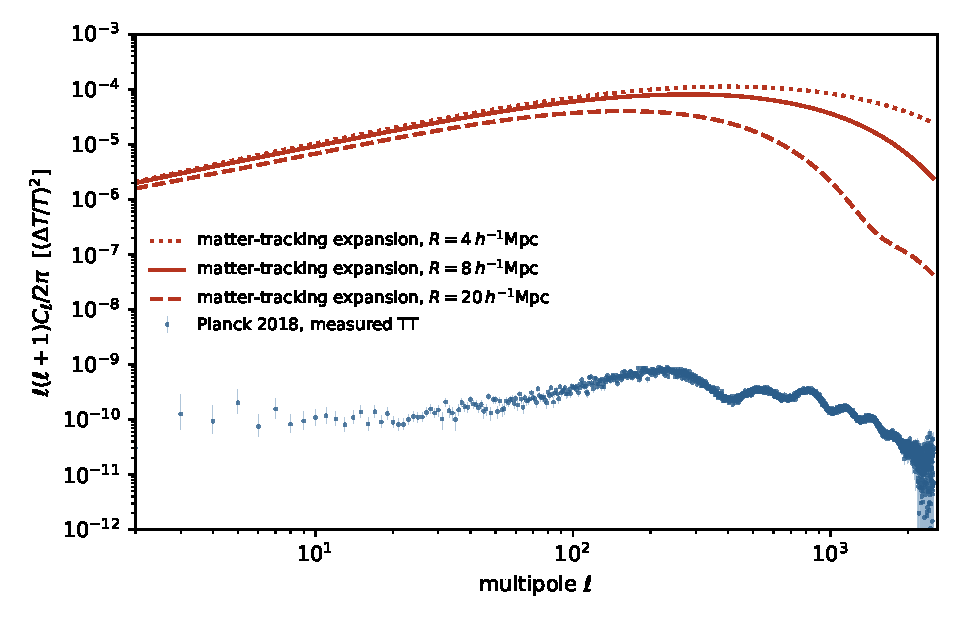
\includegraphics[width=0.8\textwidth]{fig_floor.pdf}
\caption{Angular power of the redshift anisotropy that an expansion tracking the matter distribution would produce, from~\eqref{eq:limber} on the Planck 2018 linear matter spectrum, for three smoothing radii (red), against the temperature power spectrum Planck measures (blue)~\cite{Planck2018V}. Both are in units of $(\Delta T/T)^{2}$. The prediction exceeds the measurement at every multipole, by at least $2\times10^{4}$ for $R=4$ and $8\,h^{-1}\,\mathrm{Mpc}$, and by at least $800$ for $R=20\,h^{-1}\,\mathrm{Mpc}$, where the smoothing begins to remove the smallest angular scales.}
\label{fig:floor}
\end{figure}

The choice of $R$ does not rescue the hypothesis. The radius is the scale on which the rate is taken to follow the density, and the rms falls slowly as it grows: $1.9\times10^{-2}$ at $R=4$, $1.1\times10^{-2}$ at $20$, $6.0\times10^{-3}$ at $50$, $3.3\times10^{-3}$ at $100$ and $9.6\times10^{-4}$ at $300\,h^{-1}\,\mathrm{Mpc}$---still $24$ times the whole measured anisotropy at a smoothing scale far above any on which the matter is inhomogeneous\rcpt{P04_redshift_isotropy_floor}. As the radius grows, the smoothing removes the small angular scales and the excess moves to the large ones: at $R=50$ and $100\,h^{-1}\,\mathrm{Mpc}$ the predicted power still exceeds the measured power at every multipole to $\ell=2500$, and at $R=300\,h^{-1}\,\mathrm{Mpc}$ it exceeds it at every multipole up to $\ell\approx490$, by more than a factor of $60$ up to $\ell=100$\rcpt{P04_the_floor_exceeds_the_measured_temperature_spectrum_at_every_multipole_and_the_exclusion_moves_to_low_multipoles_only_at_large_smoothing}.

\subsection{Why the number is a floor}

Each approximation in the estimate lowers it:
\begin{itemize}
\item \emph{The coefficient.} The full matter coefficient $1/3$ is retained; dropping it would treble the estimate.
\item \emph{Growth.} The contrast is weighted by its linear growth along the path, which suppresses it at high redshift, where most of the path lies; holding $\sigma_R$ at its present value along the whole path would give an estimate nearly ten times larger.
\item \emph{Linear theory.} The matter contrast on the scales that dominate~\eqref{eq:sigmapath} is nonlinear at low redshift, where nonlinear growth raises the small-scale power above the linear spectrum used here; the void and wall contrasts the backreaction programmes invoke are of order unity.
\item \emph{The local rate.} Equation~\eqref{eq:localrate} is the linear limit of the separate-universe rate; the exact rate of a nonlinear underdensity departs from the mean by more, not less.
\item \emph{The comparison.} The measured anisotropy includes the primary acoustic signal, which the hypothesis does not remove; the redshift scatter it predicts must fit inside the measured power together with everything else on the sky, so comparing it with the whole measured spectrum, as though the primordial and Sachs--Wolfe contributions were absent, understates the exclusion.
\end{itemize}
The value~\eqref{eq:value} carries the correlations of the matter field along the ray, which the measured spectrum shows and structure formation in general relativity requires. The most accommodating value drops them: light crossing statistically independent cells of uniform density, each of comoving length $R$ and with its own contrast $\sigma_R(z)$, as many of them as the finite distance to last scattering holds---$N=\chi_*/R\approx1200$ at $R=8\,h^{-1}\,\mathrm{Mpc}$---so that the scatter averages down as far as the observable universe allows. Each cell adds $gR\,\delta_R$ to~\eqref{eq:lineint}, independent contributions add in variance, and
\begin{equation}
\sigma^{2}_{\mathrm{cells}} = \int_0^{\chi_*} d\chi\; g^{2}(\chi)\,R\,\sigma_R^{2}(z)
\label{eq:floor}
\end{equation}
gives $\sigma_{\mathrm{cells}}\simeq8.9\times10^{-3}$, still some $220$ times the whole measured anisotropy\rcpt{P04_redshift_isotropy_floor}. That value is unrealistically uniform, and the rise from it to~\eqref{eq:value} is a theorem rather than a caution: for $N$ cells of average pairwise correlation $\bar\rho$ the variance of their sum is $N\sigma^{2}(1+(N-1)\bar\rho)$, which exceeds the independent value for every $\bar\rho>0$ and falls below it only for $\bar\rho<0$\rcpt{R2_the_papers_correlation_figures_are_the_ones_nothing_checked}\ldg{probability}. Gravitational clustering produces positive correlations along the line of sight, so the expectation general relativity itself supplies for the matter field moves the prediction further from the measured sky, not toward it.

The rms comparison sets an anisotropy, the scatter across directions, against~\eqref{eq:sigmapath} and~\eqref{eq:floor}, which are variances along one ray. The two differ only for modes longer than the path: every sightline is cast from the same observer, so a mode much longer than the observable region takes one value over the whole of it, lands on every direction alike, and is removed with the monopole. Measured, the across-sky scatter tracks the single-ray variance to $1\%$ for modes much shorter than the path and falls to $2\times10^{-4}$ of it for modes much longer\ldg{harmonic_analysis}; on a CDM spectrum the fraction of the single-ray variance lying in modes longer than the path is $3\times10^{-6}$, and $95\%$ of it lies in modes at least seventy times shorter, so the single-ray variance is the across-sky scatter everywhere the variance actually lives\rcpt{R50_the_long_wavelength_bullet_reverses_for_the_observable_and_the_corner_is_three_parts_per_million}\ldg{probability}. The angular power~\eqref{eq:limber} makes the same comparison directly, direction against direction. The Limber approximation is inaccurate at the lowest multipoles, by tens of per cent at $\ell\lesssim10$, which is immaterial against margins of four orders of magnitude; \eqref{eq:sigmapath} rests on the same narrow-correlation approximation along the ray, which holds because the correlation length of the smoothed field is short against the distances over which $g$ and $P$ change.

\emph{The comparison is a lower bound against an upper limit, which is what makes it robust rather than close}: the measured anisotropy bounds from above whatever redshift scatter the sky carries, and every free choice in the estimate pushes the two further apart, so the exclusion cannot be weakened by a different estimate, only by a different physical claim\ldg{statistics_inference}. For even the most accommodating value merely to reach the measured anisotropy, the sky would have to be some $220$ times more anisotropic than it is. The hypothesis that the expansion rate is locally set by the matter distribution is therefore excluded, and not marginally.

\subsection{Distinct from the Sachs--Wolfe effect}\label{sec:sw}

It is essential that this is a distinct effect from the Sachs--Wolfe and integrated Sachs--Wolfe anisotropies~\cite{Sachs1967, Rees1968}, not a re-derivation of them. When the matter's lumpiness clusters upon a single background $a(t)$, it is carried by a metric potential $\Phi$. In~\eqref{eq:redshiftrate} the local expansion of the matter still varies with its density, but the shear term no longer vanishes, and to linear order the two combine into a total derivative along the ray: the redshift a photon gains descending into a potential well is returned climbing out, the contributions \emph{telescope}, and what remains is the endpoint potential ($\sim\!10^{-5}$) and the small integrated term, with no $\sqrt{N}$ accumulation. The floor computed here is the contrary case---a genuine differential \emph{expansion}, a cosmological redshift that accumulates because there is nothing to cancel against. The observed anisotropy thus selects the telescoping, uniform-expansion picture over the accumulating, differential one. The isotropy of the CMB is not accounted for by large-scale statistical homogeneity~\cite{Scrimgeour2012}---that homogeneity is fully consistent with the differential-expansion hypothesis, which would still produce the scatter of~\eqref{eq:value}---but by uniform expansion in a cosmic time.

It is the scatter, not the mean, that is at issue. The redshift along a long ray may track the volume-averaged expansion~\cite{Rasanen2009}; the floor is the fluctuation about that average, computed. Under a matter-tracking rate it is of order $10^{-2}$ along each ray, and it is this direction-to-direction scatter, not the mean redshift, that the measured isotropy excludes.

A differential-expansion programme can evade the floor only by requiring the local rates to average to a common value in every direction: a uniform large-scale Hubble flow. But that requirement is itself a global uniform expansion in a cosmic time, the very structure such programmes set out to dispense with; imposing it to recover the observed isotropy reinstates the cosmic rest frame and the objective simultaneity it carries. Either way, the observed isotropy of the CMB redshift forces a uniform cosmic expansion.

\subsection{Timescape}\label{sec:timescape}

The timescape model of \S\ref{sec:backreaction} falls inside the hypothesis, its void and wall rates differing by a third. Its postulate that each region measures the same rate in its own proper time does not remove the differential expansion from the redshift. By~\eqref{eq:redshiftrate} a photon crossing a region gains the local rate per unit of local proper time, and per unit of volume-average time it spends less local proper time crossing a wall than a void; the redshift it gains per unit of volume-average time is therefore the region's own rate, $H_{\rm v}$ or $H_{\rm w}$, while the clock rates enter only at the ends of the path, through the acceleration term. The mean of that accumulation is exactly the model's own redshift relation~\cite{Wiltshire2009} (its eq.~38), and its scatter is of the floor's kind: for void and wall cells drawn independently along each ray, the most accommodating case, the rms of $\ln(1+z)$ across directions is $2.4\times10^{-2}$, $4.2\times10^{-2}$ and $5.4\times10^{-2}$ for cells of $10$, $30$ and $50\,h^{-1}$\,Mpc, some $600$ to $1300$ times the whole measured anisotropy\rcpt{P04_the_timescape_model_falls_inside_the_hypothesis_because_its_clock_postulate_does_not_keep_the_differential_expansion_out_of_the_redshift}. Its variance is the backreaction $\mathcal{Q}$ integrated along the ray, weighted by the time light takes to cross each cell: the term that gives the model its acceleration is the term that scatters its redshifts. The timescape papers compute observables on the average geometry~\cite{Wiltshire2009, NazerWiltshire2015, Seifert2025} and do not compute this scatter. Uniformity in local proper time is not uniformity along the journey of the light, and it is the latter that the isotropy of the CMB measures.

\section{What the exclusion establishes}\label{sec:establishes}

The floor closes the statistical escape, and one further escape is logically available and must be closed separately. A finely tuned, spherically symmetric inhomogeneity centred on the observer would produce isotropic redshift about us with no global uniform expansion; being structured rather than statistical, it is not touched by the floor. It is closed instead by the Copernican principle together with the independent isotropy of the \emph{expansion history} itself: standard rulers (baryon acoustic oscillations~\cite{Eisenstein2005}) and standard candles (Type~Ia supernovae~\cite{Riess1998, Perlmutter1999}) reconstruct the expansion along many directions and agree across the sky, so the uniformity is not the vantage artefact of a privileged centre~\cite{Barrett2000, Clarkson2010, Maartens2011}. Gpc-scale voids centred on us, the form this escape takes in the literature, are excluded directly by the kinetic Sunyaev--Zel'dovich effect and by the combined distance data~\cite{ZhangStebbins2011, Moss2011}. With the statistical alternative excluded by the floor and the centred one by the Copernican step, the disjunction is exhausted: the observed isotropy forces uniform cosmic expansion.

What that exclusion reaches is the point of the paper. The region the data reject is not a parameter corner but the entire class of histories lacking a single global scale factor on a single global time. To reject that class is to select a global, time-ordered expansion, which is the cosmic foliation made dynamical. And by \S\ref{sec:order} the foliation is logically prior to everything else the standard model assumes---``space'' is one of its slices, ``expansion'' an ordered family of them, ``isotropy'' and ``homogeneity'' properties of a slice---none of which is even statable until the foliation is in hand. A single datum therefore establishes, from the bottom up, the cosmic time on which the rest stands, the uniformity of the expansion on its slices, and---within the observable region and under the Copernican principle---the maximal symmetry of those slices. The model's foundational kinematics are not idealizations the data tolerate; they are what the data force, the one coherent alternative excluded.

Unlike the stability arguments of \S\ref{sec:tension}, the floor does not assume a Friedmann structure in its input; it derives the uniformity of the expansion from the redshift isotropy directly, a datum prior to any slice. This settles the standing dispute over backreaction structurally and from outside it: the uniform expansion that one side assumes and the other questions is fixed by measurement whichever way the averaging argument is settled, so the most rigorous defence of the standard treatment is found to presuppose the very structure the measurement supplies, and the backreaction question, however it resolves dynamically, cannot reach the foliation the floor has fixed. Were the backreaction case to carry genuine large-scale content, it would enter on that merit and against this result; it does not enter as the ground of the uniform expansion, which the measurement has removed from its reach.

The scope is worth marking. This contradicts none of the standard model's fitted predictions; with its assumptions in place it reproduces the observed expansion history, which is why it stands. What the measurement changes is the standing of those assumptions: the cosmic time and the uniformity of its expansion are forced from the bottom up, prior to and independently of the dynamical fit. The temporal claim---uniform expansion throughout the history probed---is clean, being the integral from decoupling to the present along the observed rays; the extension to a globally maximally symmetric space rests on the Copernican principle and extrapolates beyond the directly constrained region. And what the isotropy measures is the uniformity of the expansion rate along the observed rays; it does not measure, and this paper does not claim, anything about which geometry carries that expansion or how the matter within it is arranged. Nor does the measurement install a replacement: the positive account, that the expansion is set by the cosmological constant alone with the matter density a reading of cosmic epoch~\cite{JanzenCRframework}, is motivated by this forcing but not compelled by it, and is left to the companion framework rather than asserted here.

\section{What stands and what falls}\label{sec:stands}

The floor constrains the expansion \emph{rate}, not the matter content. CR's real space is locally curved and inhomogeneous---the matter density is the bend of the spatial cut off the de~Sitter vacuum profile~\cite{JanzenOperator, JanzenRange}---and that lumpiness is untouched by the argument. What is excluded is an inhomogeneous expansion rate \emph{tracking} the lumpiness: the layer advances uniformly in cosmic time while its intrinsic geometry carries the bend. Uniform expansion and lumpy matter are consistent.

The measurement leaves two things standing. The curvature stands in full: the lumpiness curves spacetime, and that curvature is the potential $\Phi$ of \S\ref{sec:sw}, whose effect on the redshift telescopes along each ray. The Friedmann equation~\eqref{eq:friedmann} stands as a relation between averages, the mean density and the rate on a slicing already given. What does not stand is the step between them, the local form of \S\ref{sec:twoforms}: that the density sets the rate region by region. The Raychaudhuri equation~\eqref{eq:raychaudhuri} is not what fails; it holds in every solution of general relativity. What fails is the claim that the rate light records is the matter's local expansion. The standard model's own perturbation theory is consistent with the floor for exactly this reason: the matter's local expansion varies with its density, but the shear that general relativity pairs with it cancels the variation out of the redshift, so the rate the light records is the uniform rate at which the slices of cosmic time advance. The curvature of the matter rides on that advance instead of setting it.

What does set the rate is then the global form of the principle. In the Friedmann models it is the average density on the slice, however lumpy the matter is on it, and the cosmic time and slices that form presupposes now rest on measurement rather than on posit. One qualification belongs here, because the companion framework's cosmology sits inside it. The Friedmann models add a posit beyond the cosmic time itself: that the slices of constant cosmic time are orthogonal to the matter's worldlines, so that cosmic time is the proper time of the matter. Strictly, the redshift relation the measurement constrains does not by itself require this. It is also satisfied by a special non-synchronous case, in which every comoving worldline crosses the slices of uniform expansion in the same way, the slices being tilted from the matter's rest frame; an example whose scale factor is identical to that of flat $\Lambda$CDM is given in~\cite{Janzen2015}. On the metric of that example the comoving congruence is sheared, and null geodesics of that metric would return an anisotropic redshift; the case reproduces the observed isotropy only when the light is assigned to a different congruence, the worldlines at rest in the slices, by a reassignment of the metric's causal structure. Events on one slice are then simultaneous and yet asynchronous in the matter's rest frame: synchrony and simultaneity come apart for the matter itself, not only for observers moving through it. That case is the cosmology the companion framework constructs, where the reassignment is selected by the limiting structure of gravitational collapse rather than chosen, and where the direction along which each slice orders its comoving worldlines is a Killing field of the metric, the static one of the Schwarzschild--de~Sitter family~\cite{JanzenCRframework}. Nothing in the present argument depends on it. What the measurement forces is the foliation and a uniform expansion on its slices, and it forces them on either reading of how the matter's rest frame stands to the slices.

The result saddles a theory without preferred frames with a preferred time, which may seem a high price to pay against the theory's elegance. Feynman's rule settles the order of priority: however beautiful a theory is, if it disagrees with experiment it is wrong~\cite{Feynman1965}. Here the disagreement does not fall on general relativity, whose equations admit the foliation the data select. It falls on two expectations about it: that no foliation would be distinguished, and that the density would set the expansion where it is.

\section{The measured foliation and what follows}\label{sec:follows}

\subsection{The order of construction reversed}\label{sec:reversed}

The construction of \S\ref{sec:order} posited a cosmic time, its slices, and their isotropy and homogeneity so that the dynamical relation~\eqref{eq:friedmann} could be stated. The measurement reverses that order. The cosmic time and the uniformity of its expansion are measured, and with the Copernican principle so are the isotropy and homogeneity of its slices, while the local form of the dynamical principle, the one form that could have been tested without them, is what fails. The cosmic-time variable was put in by hand at the outset, assumed in Einstein's 1917 cosmology and carried through Friedmann's expanding solutions to the present model, where a single global scale factor on a single global time is the background fixed before any matter is placed upon it; that foundational structure is here measured. And the direction of determination of \S\ref{sec:history}, from the content to the rate, is reversed for the \emph{rate}: the rate is fixed independently of how the content is distributed, since a rate tracking the content is precisely what the measurement excludes. Whether the same reversal extends from the rate to the scale is not settled here and is taken up in a companion~\cite{JanzenCRframework}.

\subsection{The foliation in general relativity}\label{sec:foliation}

General relativity is generally covariant. A spacetime can be sliced into spacelike hypersurfaces in many ways, and the theory does not by itself make any slicing physically special. In the $3{+}1$ form of the theory~\cite{ADM1962} a slicing is described by two functions: the lapse $N$, the proper time elapsed along the normals between neighbouring slices, and the shift $N^{i}$, the motion of the spatial coordinates from one slice to the next relative to those normals. In the canonical theory both are Lagrange multipliers, freely specifiable. Numerical relativity chooses them for stability, with maximal or 1+log slicing~\cite{BaumgarteShapiro2010}, and the absence of any preferred foliation is the root of the problem of time in canonical quantum gravity~\cite{Kuchar1992, Isham1993}. Programmes that do posit a preferred foliation posit it on theoretical grounds: the constant-mean-curvature slicing that defines York's extrinsic time~\cite{York1972}, which shape dynamics takes as fundamental~\cite{Gomes2011}; the preferred foliation of Ho\v{r}ava--Lifshitz gravity~\cite{Horava2009}; and the dynamical preferred frame of Einstein--aether theory~\cite{Jacobson2001}.

In these terms, our universe has a cosmic time whose slices carry a uniform expansion: the redshift between any two comoving worldlines is the ratio of one scale factor at the cosmic times of reception and emission, whatever the direction, to the accuracy of the floor along our past light cone and, with the Copernican step of \S\ref{sec:establishes}, across each slice. The slices are the level sets of that scale factor, and so of the temperature of the CMB in its own rest frame, which is a scalar: every observer at an event recovers the same value from the angular pattern they measure, whatever their motion. The slicing is therefore invariant rather than a convention of any observer's frame. Where the matter's worldlines are orthogonal to the slices, as the Friedmann models posit, the expansion of the matter is the mean curvature of the slices, so slices of uniform expansion are slices of constant mean curvature: the foliation the data select is York's. How the rate of comoving clocks varies against cosmic time is a separate matter. Across the last-scattering surface the measured anisotropy bounds it at the $10^{-5}$ level of the gravitational potentials; at the observer's end it is common to every direction, so isotropy seen from one place does not by itself fix how clock rates in different regions compare today. The slicing is not chosen. It is singled out by the content of the universe and located by measurement.

\subsection{What is unchanged}\label{sec:unchanged}

All of special- and general-relativistic kinematics holds on this structure. A clock deep in a potential well runs slow by the gravitational redshift. A clock moving through the cosmic rest frame runs slow by its Lorentz factor. Observers moving relative to that frame who synchronize their clocks by light signals obtain slices tilted from the frame's own, by $vx/c^{2}$ to first order, and described on the cosmic slicing their frames carry a nonzero shift. Proper times, and the times read by relatively moving synchronized clocks, track differently, exactly as relativity requires, within a structure whose common time is measured. Local Lorentz invariance is untouched: no local experiment picks out the cosmic frame, which is identified only by the large-scale content of the universe.

\subsection{Simultaneity}\label{sec:simultaneity}

The relativity of simultaneity is a statement about synchrony---which distant clocks, set by a given convention, read the same---and it holds. The relativity of \emph{synchrony} is general, a feature of relative motion, the light postulate fixing only its magnitude~\cite{JanzenWildGoose, JanzenMisconstrue}, and it is the shift: the freedom of a moving observer to tilt the slices off the comoving normal. \emph{Simultaneity} is the separate question. It does not follow that a universe whose content distinguishes a slicing has no physically distinguished relation of simultaneity, and the data show that ours distinguishes one: the slices of constant cosmic time, on which the expansion is uniform. To read the relativity of synchrony as the denial of an objective simultaneity is a modal fallacy, the absence of a local test mistaken for the absence of a fact---the imperative's characteristic dual, established as such in the companion epistemic paper~\cite{JanzenShadowExistence, JanzenWildGoose}.

This bears directly on the arguments that draw a metaphysical conclusion from the relativity of simultaneity. Rietdijk and Putnam argued that if the simultaneity of every inertial frame---its synchrony, in the terms used here---is equally valid, events on all of them are equally real, so that the future is as determinate as the past~\cite{Rietdijk1966, Putnam1967}; Penrose's version sets two people passing in a street whose planes of simultaneity reach events in the Andromeda galaxy days apart~\cite{Penrose1989}. The premise is that no frame is physically distinguished, and Stein showed early that the relativistic structure alone does not license the conclusion~\cite{Stein1968}. What the data add is that in our universe the premise is false: the cosmic foliation is physically distinguished, by the content of the universe, and located by measurement. This does not by itself settle the metaphysics of time; it removes the physical premise these arguments rest on. G\"odel objected that a cosmic time defined by the matter depends on how the matter happens to be arranged~\cite{Godel1949}; the measurement makes that dependence an empirical matter, settled for our universe. Accounts of an objective present built on cosmic time are developed by Ellis~\cite{Ellis2006}, by Ellis and Rothman~\cite{EllisRothman2010} and by the contributors to~\cite{CraigSmith2007}. Synchrony is relative; simultaneity on the cosmic foliation is absolute, and measured.

\subsection{The augmentation}\label{sec:augmentation}

What the measurement forces is the empirical half of a structural result, and the half in hand fixes the other, so it is worth stating whole. General relativity supplies a four-geometry and field equations but does not single out which of the foliations its formalism admits is the physical one~\cite{JanzenCRframework}. The standard interpretation fills the theory's silence on which slicing is physical by collapsing two distinctions at once: it reads the relativity of simultaneity as the absence of any objective present, and it reifies the four-manifold as a thing that exists. Each is a category error of the same family as the one corrected in \S\ref{sec:decomp}---there, crediting the source alone for a fact that resides also in the intervening expansion; here, crediting the manifold for what the evolving world does. Pried apart, the two are the parts a coherent formal description of an existing, evolving world requires; and they are exactly the lapse and the shift of the $3{+}1$ split read ontologically---the Newtonian part, an absolute rate of advance, and the Einsteinian part, the relativity of synchrony, the formalism the standard reading had fused and a coherent description must hold apart.

The shift is the relativity of synchrony of \S\ref{sec:simultaneity}. The lapse is the other part: the rate of advance of the layer that exists, what the clock measures~\cite{JanzenTrope}. To deny it---to hold the four-manifold itself the existent---is to treat occurrences as existents, which on analysis smuggles a fifth, meta-temporal dimension along which the block is supposed to ``exist,'' and is incoherent as a basic description~\cite{JanzenTrope, JanzenCanonicalTime}. The two corrections are not optional glosses on the formalism; they are what makes ``a world that exists and evolves'' a statable object at all. With them restored the measured result binds: the redshift isotropy forces the foliation whose advance the lapse is---a single cosmic time on whose slices the expansion is uniform---while the relativity of synchrony, untouched, is the shift, the existent the evolving layer the foliation orders and the manifold its record.

\begin{theorem}[The necessary and sufficient augmentation]\label{thm:augmentation}
Augmenting general relativity by fixing a physical foliation and reading it ontologically---the lapse the objective rate at which the existing world advances, the shift the relativity of synchrony---is both necessary and sufficient for a coherent formal description of an existing, evolving world. \emph{Necessary:} the two parts are the pried-apart forms of the existence/occurrence and synchrony/simultaneity distinctions, and a description lacking the lapse part collapses existence into occurrence---the block reading, incoherent as a basic description. \emph{Sufficient:} the two parts close the only coherent escapes---the ``events exist'' horn to the existence/occurrence correction as a category error, the ``no objective present'' horn to the synchrony/simultaneity correction as a modal fallacy, the latter then falsified outright by the measured isotropy---leaving the layered, cosmically-timed description with no surviving alternative. The augmentation alters none of general relativity's equations; it fixes which of the foliations they admit is physical and reads that one as the existent.
\end{theorem}

\noindent The measurement is what turns this from a coherent option into a forced one: the lapse the theorem requires is the advance of a foliation that is not posited but measured, read directly off the redshift isotropy together with the uniformity of the expansion on its slices. The augmentation is thus not merely the structure a coherent description \emph{may} take but the one the world is found to realize. What the theorem does \emph{not} fix is which geometry realizes the augmented structure. It fixes that the structure is necessary and sufficient, and the measurement fixes that its necessary half obtains; which four-geometry carries it, and how matter sits on that geometry, are not settled here and are taken up in companions~\cite{JanzenCRframework, JanzenOperator, JanzenRange}. What is settled \emph{here} is the structural verdict with its necessary half measured: the two-part augmentation---the completion of the Newton--Einstein formalism the standard reading left fused---is the necessary and sufficient one.

\noindent The warrant for the theorem's two moves is worth marking, because both are ordinary scientific inference rather than appeals to taste. Diagnosing the ``events exist'' horn as a category error is a correction of what the formalism actually asserts, not a preference about it. And preferring---as the floor does---the description that \emph{requires} the observed structure over one that merely \emph{permits} it is inference to the best explanation, the same step by which any theory that predicts a datum is preferred to one that accommodates it. Neither move is peculiar to this paper, and neither is taken on authority: each is made here on its own, and a companion paper takes up the general question of when such inferences are reliable~\cite{JanzenShadowExistence}. \emph{Nothing here draws on that treatment}, which is the point---an instance reached without the general account is a case that account can later rest on without circularity; and the category-error correction of \S\ref{sec:decomp} is the same method's first turn within this paper, so the paper's measured core and its structural verdict are operations of one grounded discipline.

\subsection{The cosmic rest frame}\label{sec:restframe}

The rest frame of the CMB is located by the same radiation: our own motion through it is read directly from the dipole, $(369.82\pm0.11)$~km/s toward Crater~\cite{Planck2018I}. The dipole was predicted as the signature of that motion~\cite{PeeblesWilkinson1968}, detected~\cite{Smoot1977} and is now measured to a fraction of a per cent, and the aberration and Doppler boosting it imprints on the small-scale anisotropies confirm it as a motion~\cite{Planck2013XXVII}. Whether the mean rest frame of the matter coincides with that of the CMB is tested independently by the dipole in source counts~\cite{EllisBaldwin1984}, where an amplitude exceeding the kinematic expectation has been reported~\cite{Secrest2021, Secrest2025}. That test bears on how the matter's rest frame stands to the cosmic foliation, the question of the qualification in \S\ref{sec:stands}, and not on the uniformity of the expansion measured here.

\subsection{The history closed}\label{sec:closed}

The measurement closes the arc of \S\ref{sec:history}. What Einstein posited as an approximation on stellar velocities, what de~Sitter placed beyond physical argument, and what Eddington defended in the declared absence of evidence, is what the redshift isotropy now forces. \emph{The assumption that ran against the spirit of relativity was correct}, and the objection that it gave time ``a separate position'' was correct too---as a description of the structure, though not as a reason to reject it. The principle Friedmann drew from Einstein's model survives in its global form, now standing on a measured foundation, and fails in the local form that general relativity's locality seemed to promise. The record is worth setting down because the reasoning that abandoned this structure is still in the field's hands, and because a selection made in 1920 in the declared absence of evidence, met by a measurement in the decades after, is the pattern by which theory-choice earns its standing~\cite{JanzenShadowExistence}. The parallax of this paper's title should be read with the same care the historical case requires. Stellar parallax went undetected for two millennia and was read as telling against the Earth's motion, but before the cosmos was given depth the relevant parallax was not a conceivable measurement at all---the stars sat on a sphere and had no distances to be displaced against~\cite{JanzenShadowExistence}. The objection is post-Digges, and it is Tycho who presses it. The lesson is the one this paper's floor turns on: an absent discriminator is not an absent fact, and whether a discriminator is even available is a question about the picture in hand rather than about the world.

\section{Conclusion}\label{sec:conclusion}

The principle on which relativistic cosmology was built, that the matter determines how the universe expands, has two forms. In its global form it is stated on a cosmic time and uniform slices that must be posited first; in its local form it presupposes nothing, and predicts that the expansion light records follows the matter it crosses. The isotropy of the CMB is a measurement of the expansion the radiation crossed, not only of the surface that emitted it. Read that way, it excludes the local form: an expansion tracking the matter would imprint redshift anisotropy at the $10^{-2}$ level, exceeding the measured temperature power at every multipole Planck observes by more than four orders of magnitude at $8\,h^{-1}$\,Mpc smoothing and remaining excluded for any smoothing scale up to $300\,h^{-1}$\,Mpc. The timescape model, through its own equations, exceeds it by several hundred to a thousand times. In our universe the local matter density does not set the rate of cosmic expansion. With the observer-centred alternative closed by the Copernican principle and the isotropy of the expansion history, the data select a single global expansion in a single cosmic time, and the structure the standard model posits before its dynamics is measured. Read ontologically, that measured foliation is the lapse, the objective cosmic present, and the relativity of synchrony is the shift; fixing the foliation and reading it so is the necessary and sufficient augmentation of general relativity for a coherent description of an existing, evolving world, and its necessary half is the one measured here. The general result that no exterior temporal slicing can record a finite-time completion of gravitational collapse~\cite{JanzenBHcausality} stands on causal structure alone and needs none of this evidence; what the evidence adds is that the slicing that result concerns is not one option among many but the one the universe has let us measure. As stellar parallax once converted the Earth's motion from an interpretive option into a measured fact, the isotropy of the cosmological redshift converts the cosmic foliation from a modelling convenience into a measured feature of the world.

\begin{thebibliography}{99}

\bibitem{deSitter1917} W.~de~Sitter, \emph{On the relativity of inertia. Remarks concerning Einstein's latest hypothesis}, Proc.\ Kon.\ Ned.\ Akad.\ Wetensch.\ \textbf{19} (1917) 1217--1225.

\bibitem{Janzen2015} D.~Janzen, \emph{A critical look at the standard cosmological picture}, in \emph{Questioning the Foundations of Physics: Which of Our Fundamental Assumptions Are Wrong?}, A.~Aguirre, B.~Foster and Z.~Merali eds., Springer, Cham (2015) 103--124, arXiv:1301.5980.

\bibitem{JanzenEinsteinCosmology} D.~Janzen, \emph{Einstein's cosmological considerations}, arXiv:1402.3212.

\bibitem{JanzenCRframework} D.~Janzen, \emph{Collapsed matter must become a universe: the necessary and sufficient augmentation of general relativity into a description of structural existence, proven for gravitational collapse of any symmetry}, companion paper (P7).
\bibitem{JanzenGeometricCore} D.~Janzen, \emph{Reached through the imaginary, real by construction: the maximally symmetric substrate as the geometric--ontological core of Cosmological Relativity}, companion paper (P17).

\bibitem{JanzenBHcausality}
D.~Janzen,
\emph{The event horizon is a metric singularity: a missing definition in general relativity, and the black-hole problems it dissolves}, companion paper (P1).

\bibitem{JanzenShadowExistence}
D.~Janzen,
\emph{The shadow of existence: scientific theory-choice as an empirically grounded discipline, calibrated on the historical record and on a live programme}, companion paper (P6).

\bibitem{JanzenOperator}
D.~Janzen,
\emph{Covariance of geometries over the de Sitter substrate: the slicing operator, the vacuum kernel, and matter as the bend of the cut}, companion paper (P8).

\bibitem{JanzenRange}
D.~Janzen,
\emph{The range of the de Sitter slicing operator: surjectivity onto the symmetry-reducible sector of general relativity, the Kerr--NUT--(A)dS vacuum kernel, and the wall of inhomogeneity}, companion paper (P9).

\bibitem{Janzen2025}
D.~Janzen,
\emph{Beyond Space-Time},
(2025).

\bibitem{JanzenWildGoose}
D.~Janzen,
\emph{Albert Einstein's Wild Goose Chase},
cosmiCave.org (2025).

\bibitem{JanzenFortress}
D.~Janzen,
\emph{The Fortress of Misunderstanding Physics},
cosmiCave.org (2025).

\bibitem{Aghanim2020}
Planck Collaboration (N.~Aghanim et~al.),
\emph{Planck 2018 results.~VI.~Cosmological parameters},
Astron.~Astrophys.~\textbf{641} (2020) A6.

\bibitem{Planck2018V}
Planck Collaboration (N.~Aghanim et~al.),
\emph{Planck 2018 results.~V.~CMB power spectra and likelihoods},
Astron.~Astrophys.~\textbf{641} (2020) A5; arXiv:1907.12875.

\bibitem{Lewis2000}
A.~Lewis, A.~Challinor, and A.~Lasenby,
\emph{Efficient computation of CMB anisotropies in closed FRW models},
Astrophys.~J.~\textbf{538} (2000) 473--476; arXiv:astro-ph/9911177.

\bibitem{Ellis1971}
G.~F.~R. Ellis,
\emph{Relativistic cosmology},
in \emph{Proceedings of the International School of Physics ``Enrico Fermi'', Course 47: General Relativity and Cosmology}, R.~K. Sachs ed., Academic Press, New York (1971) 104--182; reprinted in Gen.~Rel.~Grav.~\textbf{41} (2009) 581--660.

\bibitem{EllisMaartensMacCallum2012}
G.~F.~R. Ellis, R.~Maartens, and M.~A.~H. MacCallum,
\emph{Relativistic Cosmology},
Cambridge University Press, Cambridge (2012).

\bibitem{Rasanen2009}
S.~R\"as\"anen,
\emph{Light propagation in statistically homogeneous and isotropic dust universes},
J.~Cosmol.~Astropart.~Phys.~\textbf{02} (2009) 011; arXiv:0812.2872.

\bibitem{Buchert2000}
T.~Buchert,
\emph{On average properties of inhomogeneous fluids in general relativity: dust cosmologies},
Gen.~Rel.~Grav.~\textbf{32} (2000) 105--125; arXiv:gr-qc/9906015.

\bibitem{Wiltshire2007}
D.~L. Wiltshire,
\emph{Cosmic clocks, cosmic variance and cosmic averages},
New J.~Phys.~\textbf{9} (2007) 377; arXiv:gr-qc/0702082.

\bibitem{GreenWald2014}
S.~R. Green and R.~M. Wald,
\emph{How well is our Universe described by an FLRW model?},
Class.~Quantum Grav.~\textbf{31} (2014) 234003; arXiv:1407.8084.

\bibitem{Hubble1929}
E.~Hubble,
\emph{A relation between distance and radial velocity among extra-galactic nebulae},
Proc.~Natl.~Acad.~Sci.~USA \textbf{15} (1929) 168--173.

\bibitem{Eddington1920}
A.~S. Eddington,
\emph{Space, Time, and Gravitation},
Cambridge University Press, Cambridge (1920).

\bibitem{Robertson1933}
H.~P. Robertson,
\emph{Relativistic cosmology},
Rev.~Mod.~Phys.~\textbf{5} (1933) 62--90.

\bibitem{Robertson1935}
H.~P. Robertson,
\emph{Kinematics and world-structure},
Astrophys.~J.~\textbf{82} (1935) 284--301.

\bibitem{Walker1937}
A.~G. Walker,
\emph{On Milne's theory of world-structure},
Proc.~London Math.~Soc.~(2) \textbf{42} (1937) 90--127.

\bibitem{north1965}
J.~D. North,
\emph{The Measure of the Universe: A History of Modern Cosmology},
Oxford University Press, Oxford (1965).

\bibitem{Einstein1917}
A.~Einstein,
\emph{Kosmologische Betrachtungen zur allgemeinen Relativit\"atstheorie},
Sitzungsber.~K\"onigl.~Preuss.~Akad.~Wiss.~(Berlin) (1917) 142--152.

\bibitem{Friedmann1922}
A.~Friedmann,
\emph{\"Uber die Kr\"ummung des Raumes},
Z.~Phys.~\textbf{10} (1922) 377--386.

\bibitem{Friedmann1924}
A.~Friedmann,
\emph{\"Uber die M\"oglichkeit einer Welt mit konstanter negativer Kr\"ummung des Raumes},
Z.~Phys.~\textbf{21} (1924) 326--332.

\bibitem{Eddington1930}
A.~S. Eddington,
\emph{On the instability of Einstein's spherical world},
Mon.~Not.~R.~Astron.~Soc.~\textbf{90} (1930) 668--678.

\bibitem{Robertson1929}
H.~P. Robertson,
\emph{On the foundations of relativistic cosmology},
Proc.~Natl.~Acad.~Sci.~USA \textbf{15} (1929) 822--829.

\bibitem{Raychaudhuri1955}
A.~Raychaudhuri,
\emph{Relativistic cosmology.~I},
Phys.~Rev.~\textbf{98} (1955) 1123--1126.

\bibitem{Ellis1984}
G.~F.~R. Ellis,
\emph{Relativistic cosmology: its nature, aims and problems},
in \emph{General Relativity and Gravitation}, B.~Bertotti, F.~de~Felice and A.~Pascolini eds., Reidel, Dordrecht (1984) 215--288.

\bibitem{Peebles1980}
P.~J.~E. Peebles,
\emph{The Large-Scale Structure of the Universe},
Princeton University Press, Princeton (1980).

\bibitem{Wheeler1998}
J.~A. Wheeler and K.~Ford,
\emph{Geons, Black Holes, and Quantum Foam: A Life in Physics},
W.~W.~Norton, New York (1998), p.~235.

\bibitem{Feynman1965}
R.~P. Feynman,
\emph{The Character of Physical Law},
MIT Press, Cambridge, MA (1965).

\bibitem{Lemaitre1927}
G.~Lema\^itre,
\emph{Un univers homog\`ene de masse constante et de rayon croissant rendant compte de la vitesse radiale des n\'ebuleuses extra-galactiques},
Ann.~Soc.~Sci.~Bruxelles A \textbf{47} (1927) 49--59.

\bibitem{Sachs1967}
R.~K. Sachs and A.~M. Wolfe,
\emph{Perturbations of a cosmological model and angular variations of the microwave background},
Astrophys.~J.~\textbf{147} (1967) 73--90.

\bibitem{Ellis2006}
G.~F.~R. Ellis,
\emph{Physics in the real universe: time and spacetime},
Gen.~Rel.~Grav.~\textbf{38} (2006) 1797--1824; arXiv:gr-qc/0605049.

\bibitem{Barrett2000}
R.~K. Barrett and C.~A. Clarkson,
\emph{Undermining the cosmological principle: almost isotropic observations in inhomogeneous cosmologies},
Class.~Quantum Grav.~\textbf{17} (2000) 5047--5078; arXiv:astro-ph/9911235.

\bibitem{Clarkson2010}
C.~Clarkson, B.~Bassett, and T.~H.-C. Lu,
\emph{A general test of the Copernican principle},
Phys.~Rev.~Lett.~\textbf{101} (2008) 011301.

\bibitem{Eisenstein2005}
D.~J. Eisenstein et~al.,
\emph{Detection of the baryon acoustic peak in the large-scale correlation function of SDSS luminous red galaxies},
Astrophys.~J.~\textbf{633} (2005) 560--574; arXiv:astro-ph/0501171.

\bibitem{Riess1998}
A.~G. Riess et~al.,
\emph{Observational evidence from supernovae for an accelerating universe and a cosmological constant},
Astron.~J.~\textbf{116} (1998) 1009--1038; arXiv:astro-ph/9805201.

\bibitem{Perlmutter1999}
S.~Perlmutter et~al.,
\emph{Measurements of $\Omega$ and $\Lambda$ from 42 high-redshift supernovae},
Astrophys.~J.~\textbf{517} (1999) 565--586; arXiv:astro-ph/9812133.

\bibitem{Wiltshire2007PRL}
D.~L. Wiltshire,
\emph{Exact solution to the averaging problem in cosmology},
Phys.~Rev.~Lett.~\textbf{99} (2007) 251101.

\bibitem{Wiltshire2009}
D.~L. Wiltshire,
\emph{Average observational quantities in the timescape cosmology},
Phys.~Rev.~D~\textbf{80} (2009) 123512; arXiv:0909.0749.

\bibitem{NazerWiltshire2015}
M.~A. Nazer and D.~L. Wiltshire,
\emph{Cosmic microwave background anisotropies in the timescape cosmology},
Phys.~Rev.~D~\textbf{91} (2015) 063519; arXiv:1410.3470.

\bibitem{Seifert2025}
A.~Seifert, Z.~G. Lane, M.~Galoppo, R.~Ridden-Harper and D.~L. Wiltshire,
\emph{Supernovae evidence for foundational change to cosmological models},
Mon.~Not.~R.~Astron.~Soc.~\textbf{537} (2025) L55; arXiv:2412.15143.

\bibitem{Weyl1923}
H.~Weyl,
\emph{Zur allgemeinen Relativit\"atstheorie},
Phys.~Z.~\textbf{24} (1923) 230; English translation in Gen.~Rel.~Grav.~\textbf{41} (2009) 1661.

\bibitem{EGS1968}
J.~Ehlers, P.~Geren, and R.~K. Sachs,
\emph{Isotropic solutions of the Einstein--Liouville equations},
J.~Math.~Phys.~\textbf{9} (1968) 1344.

\bibitem{Stoeger1995}
W.~R. Stoeger, R.~Maartens, and G.~F.~R. Ellis,
\emph{Proving almost-homogeneity of the universe: an almost Ehlers--Geren--Sachs theorem},
Astrophys.~J.~\textbf{443} (1995) 1.

\bibitem{Nilsson1999}
U.~S. Nilsson, C.~Uggla, J.~Wainwright, and W.~C. Lim,
\emph{An almost isotropic cosmic microwave temperature does not imply an almost isotropic universe},
Astrophys.~J.~Lett.~\textbf{522} (1999) L1.

\bibitem{PeeblesWilkinson1968}
P.~J.~E. Peebles and D.~T. Wilkinson,
\emph{Comment on the anisotropy of the primeval fireball},
Phys.~Rev.~\textbf{174} (1968) 2168.

\bibitem{Smoot1977}
G.~F. Smoot, M.~V. Gorenstein, and R.~A. Muller,
\emph{Detection of anisotropy in the cosmic blackbody radiation},
Phys.~Rev.~Lett.~\textbf{39} (1977) 898.

\bibitem{Planck2018I}
Planck Collaboration (N.~Aghanim et~al.),
\emph{Planck 2018 results.~I.~Overview and the cosmological legacy of Planck},
Astron.~Astrophys.~\textbf{641} (2020) A1.

\bibitem{Planck2013XXVII}
Planck Collaboration (N.~Aghanim et~al.),
\emph{Planck 2013 results.~XXVII.~Doppler boosting of the CMB: Eppur si muove},
Astron.~Astrophys.~\textbf{571} (2014) A27.

\bibitem{EllisBaldwin1984}
G.~F.~R. Ellis and J.~E. Baldwin,
\emph{On the expected anisotropy of radio source counts},
Mon.~Not.~R.~Astron.~Soc.~\textbf{206} (1984) 377.

\bibitem{Secrest2021}
N.~J. Secrest et~al.,
\emph{A test of the cosmological principle with quasars},
Astrophys.~J.~Lett.~\textbf{908} (2021) L51.

\bibitem{Secrest2025}
N.~J. Secrest, S.~von Hausegger, M.~Rameez, R.~Mohayaee, and S.~Sarkar,
\emph{Colloquium: The cosmic dipole anomaly},
Rev.~Mod.~Phys.~\textbf{97} (2025) 041001.

\bibitem{Buchert2008}
T.~Buchert,
\emph{Dark Energy from structure: a status report},
Gen.~Rel.~Grav.~\textbf{40} (2008) 467.

\bibitem{Rasanen2004}
S.~R\"as\"anen,
\emph{Dark energy from back-reaction},
J.~Cosmol.~Astropart.~Phys.~\textbf{02} (2004) 003.

\bibitem{Kolb2006}
E.~W. Kolb, S.~Matarrese, and A.~Riotto,
\emph{On cosmic acceleration without dark energy},
New J.~Phys.~\textbf{8} (2006) 322.

\bibitem{Clarkson2011}
C.~Clarkson, G.~Ellis, J.~Larena, and O.~Umeh,
\emph{Does the growth of structure affect our dynamical models of the universe? The averaging, backreaction and fitting problems in cosmology},
Rep.~Prog.~Phys.~\textbf{74} (2011) 112901.

\bibitem{BuchertRasanen2012}
T.~Buchert and S.~R\"as\"anen,
\emph{Backreaction in late-time cosmology},
Annu.~Rev.~Nucl.~Part.~Sci.~\textbf{62} (2012) 57.

\bibitem{GreenWald2011}
S.~R. Green and R.~M. Wald,
\emph{A new framework for analyzing the effects of small scale inhomogeneities in cosmology},
Phys.~Rev.~D \textbf{83} (2011) 084020.

\bibitem{Buchert2015}
T.~Buchert et~al.,
\emph{Is there proof that backreaction of inhomogeneities is irrelevant in cosmology?},
Class.~Quantum Grav.~\textbf{32} (2015) 215021.

\bibitem{Rees1968}
M.~J. Rees and D.~W. Sciama,
\emph{Large-scale density inhomogeneities in the universe},
Nature \textbf{217} (1968) 511.

\bibitem{Scrimgeour2012}
M.~I. Scrimgeour et~al.,
\emph{The WiggleZ Dark Energy Survey: the transition to large-scale cosmic homogeneity},
Mon.~Not.~R.~Astron.~Soc.~\textbf{425} (2012) 116.

\bibitem{Maartens2011}
R.~Maartens,
\emph{Is the Universe homogeneous?},
Phil.~Trans.~R.~Soc.~A \textbf{369} (2011) 5115.

\bibitem{ZhangStebbins2011}
P.~Zhang and A.~Stebbins,
\emph{Confirmation of the Copernican principle at Gpc radial scale and above from the kinetic Sunyaev--Zel'dovich effect power spectrum},
Phys.~Rev.~Lett.~\textbf{107} (2011) 041301.

\bibitem{Moss2011}
A.~Moss, J.~P. Zibin, and D.~Scott,
\emph{Precision cosmology defeats void models for acceleration},
Phys.~Rev.~D \textbf{83} (2011) 103515.

\bibitem{EllisRothman2010}
G.~F.~R. Ellis and T.~Rothman,
\emph{Time and spacetime: the crystallizing block universe},
Int.~J.~Theor.~Phys.~\textbf{49} (2010) 988.

\bibitem{CraigSmith2007}
W.~L. Craig and Q.~Smith, eds.,
\emph{Einstein, Relativity and Absolute Simultaneity},
Routledge, London (2007).

\bibitem{Godel1949}
K.~G\"odel,
\emph{A remark about the relationship between relativity theory and idealistic philosophy},
in \emph{Albert Einstein: Philosopher-Scientist}, P.~A. Schilpp ed., Library of Living Philosophers, Evanston (1949) 555.

\bibitem{York1972}
J.~W. York,
\emph{Role of conformal three-geometry in the dynamics of gravitation},
Phys.~Rev.~Lett.~\textbf{28} (1972) 1082.

\bibitem{Limber1953}
D.~N. Limber,
\emph{The analysis of counts of the extragalactic nebulae in terms of a fluctuating density field},
Astrophys.~J.~\textbf{117} (1953) 134.

\bibitem{ADM1962}
R.~Arnowitt, S.~Deser and C.~W. Misner,
\emph{The dynamics of general relativity},
in \emph{Gravitation: An Introduction to Current Research}, L.~Witten ed., Wiley, New York (1962) 227; arXiv:gr-qc/0405109.

\bibitem{BaumgarteShapiro2010}
T.~W. Baumgarte and S.~L. Shapiro,
\emph{Numerical Relativity: Solving Einstein's Equations on the Computer},
Cambridge University Press, Cambridge (2010).

\bibitem{Kuchar1992}
K.~V. Kucha\v{r},
\emph{Time and interpretations of quantum gravity},
in \emph{Proceedings of the 4th Canadian Conference on General Relativity and Relativistic Astrophysics}, G.~Kunstatter, D.~E. Vincent and J.~G. Williams eds., World Scientific, Singapore (1992) 211.

\bibitem{Isham1993}
C.~J. Isham,
\emph{Canonical quantum gravity and the problem of time},
in \emph{Integrable Systems, Quantum Groups, and Quantum Field Theories}, L.~A. Ibort and M.~A. Rodr\'iguez eds., Kluwer, Dordrecht (1993) 157; arXiv:gr-qc/9210011.

\bibitem{Gomes2011}
H.~Gomes, S.~Gryb and T.~Koslowski,
\emph{Einstein gravity as a 3D conformally invariant theory},
Class.~Quantum Grav.~\textbf{28} (2011) 045005; arXiv:1010.2481.

\bibitem{Horava2009}
P.~Ho\v{r}ava,
\emph{Quantum gravity at a Lifshitz point},
Phys.~Rev.~D~\textbf{79} (2009) 084008; arXiv:0901.3775.

\bibitem{Jacobson2001}
T.~Jacobson and D.~Mattingly,
\emph{Gravity with a dynamical preferred frame},
Phys.~Rev.~D~\textbf{64} (2001) 024028; arXiv:gr-qc/0007031.

\bibitem{Rietdijk1966}
C.~W. Rietdijk,
\emph{A rigorous proof of determinism derived from the special theory of relativity},
Phil.~Sci.~\textbf{33} (1966) 341.

\bibitem{Putnam1967}
H.~Putnam,
\emph{Time and physical geometry},
J.~Philos.~\textbf{64} (1967) 240.

\bibitem{Stein1968}
H.~Stein,
\emph{On Einstein--Minkowski space-time},
J.~Philos.~\textbf{65} (1968) 5.

\bibitem{Penrose1989}
R.~Penrose,
\emph{The Emperor's New Mind},
Oxford University Press, Oxford (1989).

\bibitem{CollinsHawking1973}
C.~B. Collins and S.~W. Hawking,
\emph{The rotation and distortion of the Universe},
Mon.~Not.~R.~Astron.~Soc.~\textbf{162} (1973) 307.

\bibitem{Saadeh2016}
D.~Saadeh, S.~M. Feeney, A.~Pontzen, H.~V. Peiris and J.~D. McEwen,
\emph{How isotropic is the Universe?},
Phys.~Rev.~Lett.~\textbf{117} (2016) 131302; arXiv:1605.07178.

\bibitem{Zhou2025}
A.~J. Zhou, S.~Dodelson and D.~Scolnic,
\emph{The isotropy of cosmic expansion in the early and late Universe},
arXiv:2506.14878 (2025).

\bibitem{JanzenCanonicalTime}
D.~Janzen,
\emph{The canonical problem of time as a category error: an empirically forced cosmic time, deparametrization, the dissolution of frozen dynamics, and a graviton quantization the de~Sitter horizon closes without a free parameter---the seam where $\hbar$ enters gravity---in Cosmological Relativity}, companion paper (P10).
\bibitem{JanzenMisconstrue}
D.~Janzen,
\emph{Did Einstein Misconstrue Relativity's Real Meaning?},
cosmiCave.org (2025).
\bibitem{JanzenTrope}
D.~Janzen,
\emph{Time Travel: A Five-Dimensional Trope},
cosmiCave.org (2025).
\bibitem{JanzenCosmogenesis} D.~Janzen, \emph{Cosmogenesis: the Big Bang as a synthesis of Cosmological Relativity's deductively forced consequences, and the primordial light-element abundances it produces}, companion paper (P16).

\bibitem{Bessel1838}
F.~W. Bessel,
\emph{Bestimmung der Entfernung des 61sten Sterns des Schwans},
Astron.~Nachr.~\textbf{16} (1838) 65--96.
\end{thebibliography}


\clearpage
\section*{Appendix R\quad Computational Receipts}\label{app:receipts}
\addcontentsline{toc}{section}{Appendix R: Computational Receipts}
\small\noindent Each computation marked \rcptmarker\ in the text is verified by a runnable receipt in the \texttt{receipts/} directory that ships with this work; status \textsf{OK} = verified (traced, run, output matches the claim). This appendix is generated from the receipt index, not maintained by hand.\par\medskip
\begingroup\renewcommand{\arraystretch}{1.25}
\begin{description}
\item[\rcptlabel{P04_redshift_isotropy_floor}{P4R1}\textbf{P4R1}\quad\texttt{P04\_redshift\_isotropy\_floor}]\hfill\textsf{[OK]}\\
\textit{sec:floor} \ (redshift-isotropy floor: light crossing independent uniform cells of length R = 8 h\textasciicircum{}-1 Mpc, each expanding at its own rate H(1 - f delta/3), accumulates a redshift scatter of 1.6e-2 with the matter field's correlations along the ray (8.9e-3 for independent cells, the most accommodating case), some 390 (220) times the whole measured CMB anisotropy 4.1e-5, from the measured Planck 2018 TT spectrum -> matter-tracking expansion excluded). 
\emph{Computes:} CAMB on the Planck 2018 base parameters (sigma\_8 0.811, z\_* 1089.9; growth rate read at k = 1e-3 h/Mpc); g = aHf/3; uncorrelated int dchi g\textasciicircum{}2 R sigma\_R\textasciicircum{}2 and correlated int dchi g\textasciicircum{}2 (1/2pi) int dk k P\_R for R = 4..300; \textasciitilde{}1200 cells at R = 8; measured TT rms l = 2..2508; genuine-floor (correlation and growth weighting both raise it) + a density-independent rate gives zero
 \emph{Bound:} linear separate-universe rate taken as the hypothesis; the comparator is the measured spectrum
\ \emph{Run:} \texttt{python3 receipts/P04\_modern\_parallax/P04\_redshift\_isotropy\_floor.py}
\item[\rcptlabel{P04_the_floor_exceeds_the_measured_temperature_spectrum_at_every_multipole_and_the_exclusion_moves_to_low_multipoles_only_at_large_smoothing}{P4R2}\textbf{P4R2}\quad\texttt{P04\_the\_floor\_exceeds\_the\_measured\_temperature\_spectrum\_at\_every\_multipole\_and\_the\_exclusion\_moves\_to\_low\_multipoles\_only\_at\_large\_smoothing}]\hfill\textsf{[OK]}\\
\textit{sec:floor, fig:floor} \ (the floor multipole by multipole against Planck's MEASURED TT spectrum: the Limber angular power of a matter-tracking expansion exceeds the measured power at every multipole from l = 2 to 2500 by at least 2.35e4 (2e5 at the median) at R = 8 h\textasciicircum{}-1 Mpc, by at least 2.5e4 at R = 4 and 872 at R = 20; at R = 50 and 100 it still exceeds at every multipole (minima 20 and 1.3), and at R = 300 at every multipole up to l = 492, by more than 60 up to l = 100; the rms figures (8.9e-3 cells, 1.6e-2 correlated, R scan to 9.6e-4 and 24x) pinned against the measured rms 4.06e-5). 
\emph{Computes:} CAMB on the Planck 2018 base parameters; the measured PR3 TT spectrum (`P04\_floor\_data/planck\_TT\_full.txt`); the 33 high-l multipoles with non-positive measured power left out of the minimum ratios; about 30 s
 \emph{Bound:} Limber, inaccurate by tens of per cent at l <\textasciitilde{} 10, against margins of four orders
\ \emph{Run:} \texttt{python3 receipts/P04\_modern\_parallax/P04\_the\_floor\_exceeds\_the\_measured\_temperature\_spectrum\_at\_every\_multipole\_and\_the\_exclusion\_moves\_to\_low\_multipoles\_only\_at\_large\_smoothing.py}
\item[\rcptlabel{P04_the_timescape_model_falls_inside_the_hypothesis_because_its_clock_postulate_does_not_keep_the_differential_expansion_out_of_the_redshift}{P4R3}\textbf{P4R3}\quad\texttt{P04\_the\_timescape\_model\_falls\_inside\_the\_hypothesis\_because\_its\_clock\_postulate\_does\_not\_keep\_the\_differential\_expansion\_out\_of\_the\_redshift}]\hfill\textsf{[OK]}\\
\textit{sec:timescape} \ (the timescape model falls inside the hypothesis: its walls expand at two-thirds the rate of its voids in the volume-average time (Wiltshire 2009, eqs. 11, 14, 15, 38), and its clock postulate does not keep the difference out of the redshift, a photon gaining H\_v or H\_w per unit of volume-average time with the clock rates entering only at the path's ends; the mean reproduces the model's own eq. 38, and independent void/wall cells of 10, 30 and 50 h\textasciicircum{}-1 Mpc give an rms in ln(1+z) of 2.4e-2, 4.2e-2 and 5.4e-2, some 600 to 1300 times the whole measured anisotropy 4.1e-5 -> timescape excluded with the averaging programme). 
\emph{Computes:} the tracker identities, Q two ways, the eq. 38 mean and the three rms figures asserted; the analytic variance against a 4000-ray Monte Carlo within 5 per cent; under 10s
 \emph{Bound:} the most accommodating case, independent cells; correlations along the ray raise the scatter
\ \emph{Run:} \texttt{python3 receipts/P04\_modern\_parallax/P04\_the\_timescape\_model\_falls\_inside\_the\_hypothesis\_because\_its\_clock\_postulate\_does\_not\_keep\_the\_differential\_expansion\_out\_of\_the\_redshift.py}
\item[\rcptlabel{I20_the_redshift_is_a_conformal_killing_charge_on_the_null_cone}{P4R4}\textbf{P4R4}\quad\texttt{I20\_the\_redshift\_is\_a\_conformal\_killing\_charge\_on\_the\_null\_cone}]\hfill\textsf{[OK]}\\
\textit{sec:decomp} \ (I20 --- THE REDSHIFT IS A CONFORMAL-KILLING CHARGE ON THE NULL CONE. Integrable-systems field bake, probe I20. In conformal FLRW form d/deta is shown by explicit Lie derivative to be a CONFORMAL and not an exact Killing vector, so its charge is conserved only where p.p = 0; there it is a*omega, whose constancy IS 1+z = a\_obs/a\_em and whose logarithm is int H dt. Carries a MASSIVE CONTROL: the spatial momentum still falls as 1/a but a*E is not constant for m nonzero, and it recovers constancy in the massless limit -- so the null-cone restriction is load-bearing and P04's line-of-sight integral is a statement about light.). 
\emph{Computes:} runs clean; nine verdicts including a massive control that fails off the cone and recovers in the limit
 \emph{Bound:} derived here; no parameter pinned
\ \emph{Run:} \texttt{python3 receipts/P04\_modern\_parallax/I20\_the\_redshift\_is\_a\_conformal\_killing\_charge\_on\_the\_null\_cone.py}
\item[\rcptlabel{R2_the_papers_correlation_figures_are_the_ones_nothing_checked}{P4R5}\textbf{P4R5}\quad\texttt{R2\_the\_papers\_correlation\_figures\_are\_the\_ones\_nothing\_checked}]\hfill\textsf{[OK]}\\
\textit{sec:floor} \ (R2 --- P04's CORRELATION THEOREM. For N cells of average pairwise correlation rhobar along the ray the variance of their sum is N sigma\textasciicircum{}2 (1 + (N-1) rhobar), exceeding the independent value for every rhobar > 0, so the uncorrelated floor is a lower bound; checked symbolically and by simulation. CONTROL: a NEGATIVE rhobar must reduce the variance, or the positivity clause would be vacuous.). 
\emph{Computes:} runs clean; four verdicts including the sign control
 \emph{Bound:} derived here; the size of the rise on the measured spectrum is P04\_redshift\_isotropy\_floor's
\ \emph{Run:} \texttt{python3 receipts/P04\_modern\_parallax/R2\_the\_papers\_correlation\_figures\_are\_the\_ones\_nothing\_checked.py}
\item[\rcptlabel{R50_the_long_wavelength_bullet_reverses_for_the_observable_and_the_corner_is_three_parts_per_million}{P4R6}\textbf{P4R6}\quad\texttt{R50\_the\_long\_wavelength\_bullet\_reverses\_for\_the\_observable\_and\_the\_corner\_is\_three\_parts\_per\_million}]\hfill\textsf{[OK]}\\
\textit{sec:floor} \ (P04's floor and its correlated value are variances along one ray, while the bounded quantity is the scatter ACROSS directions; every sightline is cast from the same observer, so a mode longer than the observable region is a monopole and cancels out of the anisotropy -- the two agree for modes shorter than the path and part only for longer ones). 
\emph{Computes:} casts sightlines from one origin through a plane-wave Gaussian field and measures BOTH the single-ray variance and the across-sky scatter: the ratio is 0.990 at kL in 100..1000 and 2.0e-4 at kL in 0.01..0.1, monotone between, stable under halving the modes, doubling the sightlines and changing the seed; then integrates a BBKS CDM spectrum and finds only 3.1e-6 of the single-ray variance below k = 1/L, with 95 percent of it above kL = 70
 \emph{Bound:} SUPPORTS P04 -- the single-ray variance is the across-sky scatter wherever the variance lives. NOT CLAIMED: any value of the floor itself (P04\_redshift\_isotropy\_floor owns that)
\ \emph{Run:} \texttt{python3 receipts/P04\_modern\_parallax/R50\_the\_long\_wavelength\_bullet\_reverses\_for\_the\_observable\_and\_the\_corner\_is\_three\_parts\_per\_million.py}
\item[\label{rcpt:B11_three_triples_two_identifications}\textbf{}\quad\texttt{B11\_three\_triples\_two\_identifications}]\hfill\textsf{[OK]}\\
\textit{sec:cycloid} \ (THREE three-fold structures and TWO open identifications carried in two registers that do not reference each other --- the root triple is the shared vertex of both and appears in neither as such). 
\emph{Computes:} asserts all three structures at source, P4s two-triples question and its \{0,1,2\} requirement, and that neither register cites the other (8 checks)
 \emph{Bound:} NOT-A-PAPER-CLAIM --- connects two open items; no identification established
\ \emph{Run:} \texttt{python3 receipts/L221\_the\_bridge/B11\_three\_triples\_two\_identifications.py}
\item[\label{rcpt:B12_the_two_triples_are_typed_differently}\textbf{}\quad\texttt{B12\_the\_two\_triples\_are\_typed\_differently}]\hfill\textsf{[OK]}\\
\textit{sec:cycloid} \ (the two triples are NOT one structure: the ROOT triple is the f=0 locus (roots 1/sqrt3, 1/sqrt3, -2/sqrt3, sum zero) while the CAUSAL triple is three VALUES of f each with one locus --- three-element sets of different KINDS). 
\emph{Computes:} asserts P4s question and its three-equally-spaced-values clause, computes the Nariai cubics roots and zero-sum and double root, matches PO-2s two distinguished roots, and counts the loci per level (8 checks)
 \emph{Bound:} NOT-A-PAPER-CLAIM --- a NEGATIVE result discharging the corpuss only DISCOVERABLE-PROOF
\ \emph{Run:} \texttt{python3 receipts/L221\_the\_bridge/B12\_the\_two\_triples\_are\_typed\_differently.py}
\end{description}\endgroup

\ldgappendix{appendix_ledgers_P4}

\end{document}
